%!TEX root = ../Master.tex
\chapter{Problem Analysis} \label{cha:problem_analysis}

To come around the base of the Initiating problem, the report will describe and analyse different aspect which deals with the problem of navigating different user around. The aspects the report will describe can be put into groups: social relevance and users, technology and attrbutes, organization and infrastructure. In details the report will describe and analyse the social relevence and potential users with a stake in this. An overview of the technologies currently in use, and a look into their attributes will be given, and the organization and infrastructure of a hospital will be taken into consideration, for how the restriction to how the solution will be made. \kanote{skal revideres}

%!TEX root = ../../Master.tex
\section{Social Relevance}


Technology plays a major role in today's modern society and everywhere you go, you will stumble upon some form of technology. Today's society would not exist without the technological advancements which man has made in the past. Despite this fact, not all technological advancements remain relevant and not all technologies have a use in a modern society. An example of this would be the steam pump. It was once a very important invention and to a degree it still is because it laid the foundation for more advanced technology. However it became obsolete as more advanced technology has made a more advanced pump. Hence the relevancy to society of a certain technology is determined by the use it has, and whether it can compete with existing technologies in its own field.

\subsection{Navigating Today's World}
It can be a daunting task to find your way around today's modern society. Past one's comfort zone the roads may seem infinite and navigating them, an impossible task. This was previously, and still is, alleviated with the use of maps, however maps will not dynamically update your current position and reading a map can be very difficult for the inexperienced. However, in the 1980's, the world saw the advent of GPS \cite{gps_advent}. GPS navigation improved upon navigation via maps as it plans the route for the user, while at the same time dynamically updates the user position, which removed the need for the user to keep track of their position. This made the need for reading a map and planning a route superfluous. These improvements over the traditional map meant that GPS navigation would be capable of competing with the existing technology at the time (i.e. maps, compass etc.). GPS navigation has remained a relevant technology to this day because navigating around the world is just as necessary and challenging now as it has ever been.

\subsection{Navigating indoors}
GPS navigation helped make outdoor navigation easier, but the system does not work indoors, due to limitations with the signal and accuracy \cite{gps_tech}. With facilities getting larger and more complex every day, the need for indoor navigation has never been greater.

While outdoor navigation saw the advent of GPS navigation, indoor navigation has had to rely on old fashioned navigation where the user has to manually position and navigate themselves, as described in \cref{sec:anal_nav}. With the increasing use of GPS navigation, which requires little to no user action, it would seem anything but likely that people have become more skilled at manual navigation. This poses the problem of how people can navigate reliably indoors.

What makes this a problem is the fact, that if individuals cannot get to where they need to be, they cannot perform the task they set out to do. This leads to frustration for those involved, be it the visitor at a hospital or the patient awaiting a visit. While navigation may seem simple to many it is imperative to acknowledge that it becomes easier with knowledge of the area and newcomers most definitely will struggle to find their way.

Many solutions to this have been proposed and developed over time, however it remains evident that none of the solutions have managed to solve the problem to satisfaction, as proved by the continued attempts to solve the problem \cite{skejby_attempt}.

\subsection{Relevance of Better Indoor Navigation}
In recent years the Danish government has restructured and made several cutbacks to the national healthcare system in attempts to save money \cite{cutback_danNHS}, however it was done on the premise that it would not compromise on the quality of the health care provided. This means that the Danish hospitals now have to provide the same level of care for a fraction of the cost and so efficiency improvement has been a key point in the aforementioned restructuring. One of the ways the Danish hospitals have had to deal with the cutbacks is by laying off employees \cite{cutback_firing}\cite{cutback_danNHS}, this means the remaining staff (nurses etc.) have to do more in the same amount of time, so the effective use of the staff's time is crucial.

A 2004 study \cite{timewaste}\cite{timewaste_report}, researching the role of the physical environment in modern hospitals, found that in a 300-bed hospital, the staff spent around 4500 hours per year helping patients and visitors find their way around the hospital. This amounts to around 20 hours a day of time wasted, time that could potentially be saved by better indoor navigation.

With so much focus on effectiveness and saving money, this is an issue that must be considered relevant, and should a proposed solution be able to track positions dynamically it would be able to save even more time as the study also shows that a large amount of time is wasted by the staff looking for medications, patients etc.

\subsection{Summary}
The solution to this problem may not be simple as many complexities arise when dealing with different prerequisites and goals, however it is not a problem that should be overlooked as the potential gains are substantial and amount to both money and time saved and it should save many frustrations for the people as a whole.

%!TEX root = ../../Master.tex
\section{Analogue Navigation in Hospitals} % (fold 
\label{sec:anal_nav}
In this section we will discuss existing analogue navigation platforms. We will in this section describe the strengths and weaknesses of existing analogue navigation platforms, in order to use this knowledge for our solution. Our main source for \cref{sec:anal_nav} is a trip to Sygehus Nord in Aalborg. Some figures in this section, was taken during the research at Sygehus Nord. Some of the assumptions made in \cref{sec:anal_nav} are based on the information gathered during the research. 

\subsection{Signs} \label{sub:sign}

Signs can be placed that mark different areas of the hospital. \enquote{Main entrance} and \enquote{Ambulance entrance}\cite{signs_hospital} signs can be used to mark key places that the visitor can navigate from\cite{art_Osborne}. There are a standard for how some signs should look, like the AED sign\cite{Signs_AED}.
Interior signs are also placed in the hospital, they are affixed to the walls, doors or windows or hang from the ceiling. These signs serve multiple purposes; some signs will describe the sign's location, others will point to other named areas and some will do both. 
If the hospital consists of multiple buildings, they can be numbered in order to navigate people to specific buildings. See \cref{fig:signs1,fig:signs2}.

A positive thing about signs is that they can give a fast impression about where the different locations are.

Signs can be hard to spot if the visitor is not familiar with the hospital. A sign can also be obstructed by other signs or if the room/hallway is filled with people. Another problem regarding signs, is that they might be hard to use if the visitor has reading problems. If the one reading a sign cannot understand the language or is an illiterate, it becomes hard to find the information that is relevant \cite{signs_reading}. Too much information can also be displayed on signs in such a way that it becomes confusing or hard to see the system behind placement of the signs.
An example, if the visitor is in building A and wants to visit a patient in building B, floor 6. It could become a challenge to set up enough signs to guide the visitor to the right building and floor, without drowning the other visitors with irrelevant information.

\begin{figure}
\centering
  \begin{minipage}{0.45\textwidth}
    \centering
    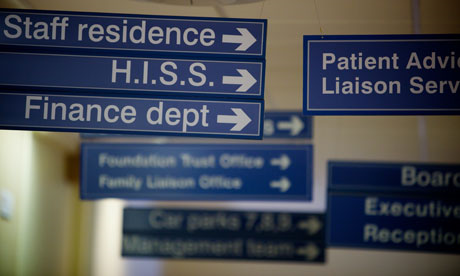
\includegraphics[width=\textwidth]{Alder-Hey-hospital-signs-007.png}
    \caption{Signs placed along a hall. \cite{signs_hospital}} \label{fig:signs1}
  \end{minipage}
  \hfill
  \begin{minipage}{0.45\textwidth}
    \centering
    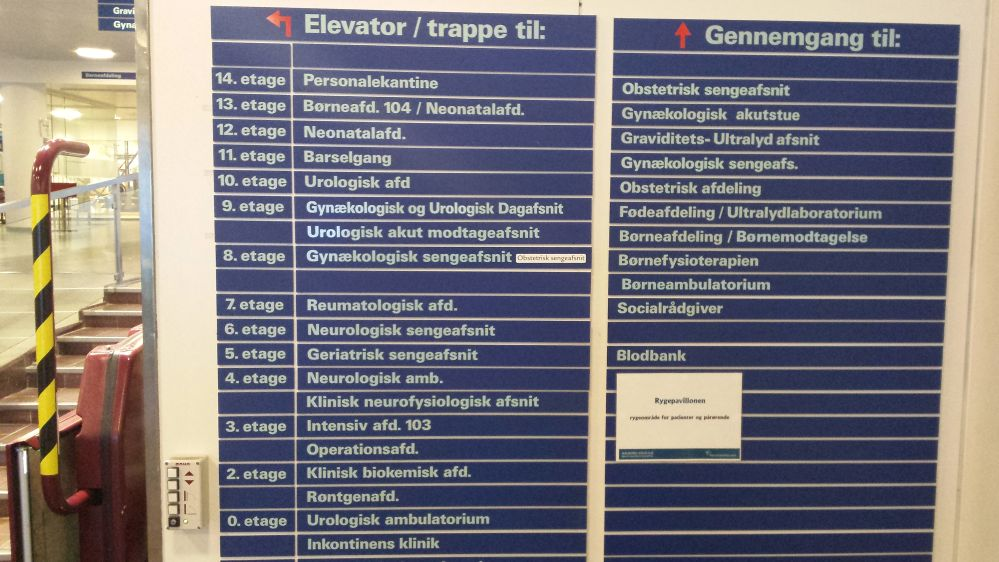
\includegraphics[width=\textwidth]{tavle.jpg}
    \caption{An overview sign of the different floors at Sygehus nord Aalborg} \label{fig:signs2}
  \end{minipage}
  \end{figure}

\subsection{Maps} \label{sub:map}
Analogue maps \cite{map} offer a top-down view of the hospital with all the different locations marked by text or colour \cite{art_Osborne}. See \cref{fig:map}. Maps can be affixed to walls or found in compact versions meant to be carried around. The stationary maps sometimes have a red dot that marks the location of the map. By knowing the current position, the visitor should be able to navigate with more ease \cite{map_survey} as they will not have to look for something recognizable that would otherwise identify their current position. If the building has multiple floors, the map will be split up into layers each depicting a floor in order to more easily represent the 3D structure.

Maps are able to efficiently show hot spots and quickly gain an overview on the location \cite{pros_analog_map}.

A common problem with maps is they can become very complicated to get an overview of if they cover multiple floors \cite{map_confusing}. If the visitor is already inside the building, it can sometimes be difficult to figure out where they are corresponding to the map. If the visitors are in a hallway it can be difficult to distinguish it from the other hallways on the map.

  \begin{figure}[ht!]
  \centering
  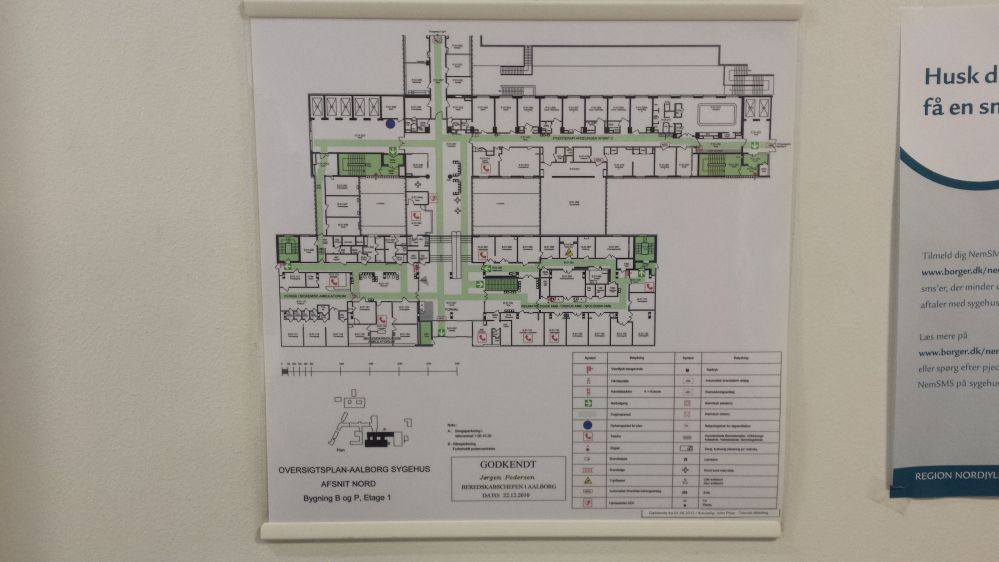
\includegraphics[width=90mm]{kortvaeg.jpg}
  \caption{A map on the wall at Sygehus nord Aalborg}
  \label{fig:map}
  \end{figure}

\subsection{Colour Coding}\label{sub:col}
Coloured stripes are lines painted on walls or floors. See \cref{fig:colour_floor}. They mark key routes to get to certain locations in the hospital. Typically a sign describing the location the colours lead to. One line might say \enquote{recovery} and if followed, will lead to the recovery department. Some departments also have an entire theme in a certain colour. In this way, it might become easier for some people to navigate the next time they visit the hospital, if they can remember the colours representing that department.
Places that use this method of navigation would seamlessly offer an easy way of letting the visitors navigate, because the information provided by the colours are very simple to understand.

A problem with colour coding is that it is very static. If for example some rooms switches their function the stripes on the wall have to be repainted which will be a lot of work. If there are stripes leading to all the different departments, the information could potentially clutch up and become confusing. This method also shares a downside together with the signs, as people with reading disorder  or the colour-blind could have trouble with this form of navigation.

\begin{figure}[htb]
  \begin{center} 
    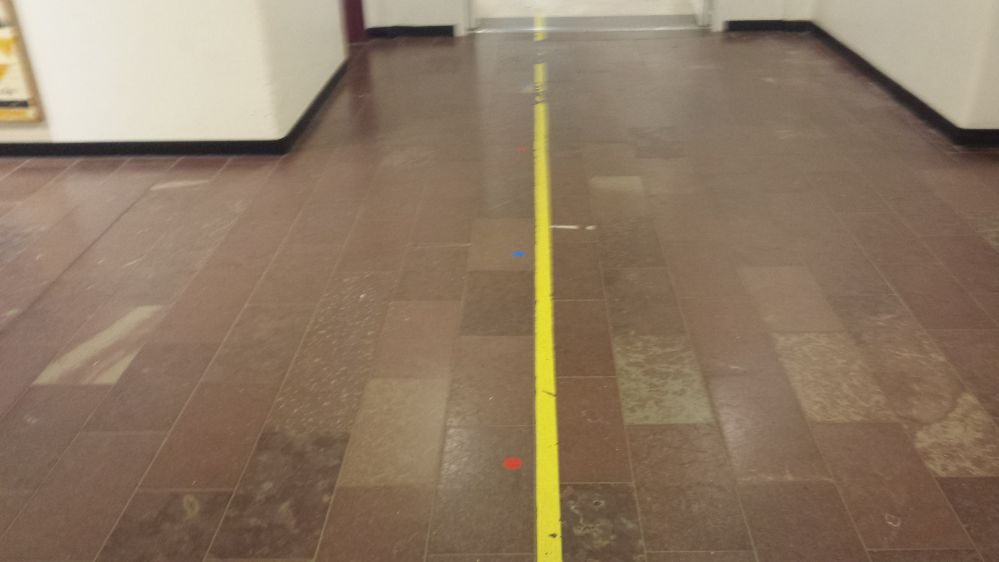
\includegraphics[width=0.5\textwidth]{stribe2.jpg}
  \end{center}
  \caption{Colour coding in use at Sygehus nord Aalborg}
  \label{fig:colour_floor}
\end{figure}




\subsection{Phone}\label{sub:pho}

Visitors are able to call the hospital's main number, and ask questions to a live operator. This can be done from any phone but there is no guarantee that a live operator is available. \cite{sign_ring}
 
The limitations regarding the phone, are high as the informer is limited by only having his/her voice as their tool. Miscommunication can occur as directions only can be delivered by words. As said before, this form of navigation strictly depends on an assigned personal to answer the phone. If no one is at the phone, it becomes utterly useless.
If the service is used often, more than one employee might be assigned to the phone. It could become an expensive service if there is a dedicated staff assigned to the phone.

\chnote{Positively providing jobs}

\subsection{Human Interaction}\label{sub:human}
Visitors can ask the staff including the receptionist regarding navigation around the hospital \cite{job}. Very much like the phone, however human interaction has an advantage of being more precise. There will be less confusion as body language can be used in the answering of the question \cite{body_vs_phone}.

At \enquote{Sygehus Nord Aalborg} a receptionist booth is located at the main entrance. See \cref{fig:rec_booth}. If the visitor arrives at an entrance different from the main one, they might not know where the receptionist is if they need help. The information received from the receptions have to be memorized when the visitor ventures away from the desk. This means that directions could become hard to remember if they have to get to a distant location inside the building. A way the receptionist could help the visitor remember, would be to write a note but even so the text could be misunderstood \chnote{misperceived.} or in other ways mixed up.

  \begin{figure}[ht!]
    \centering
    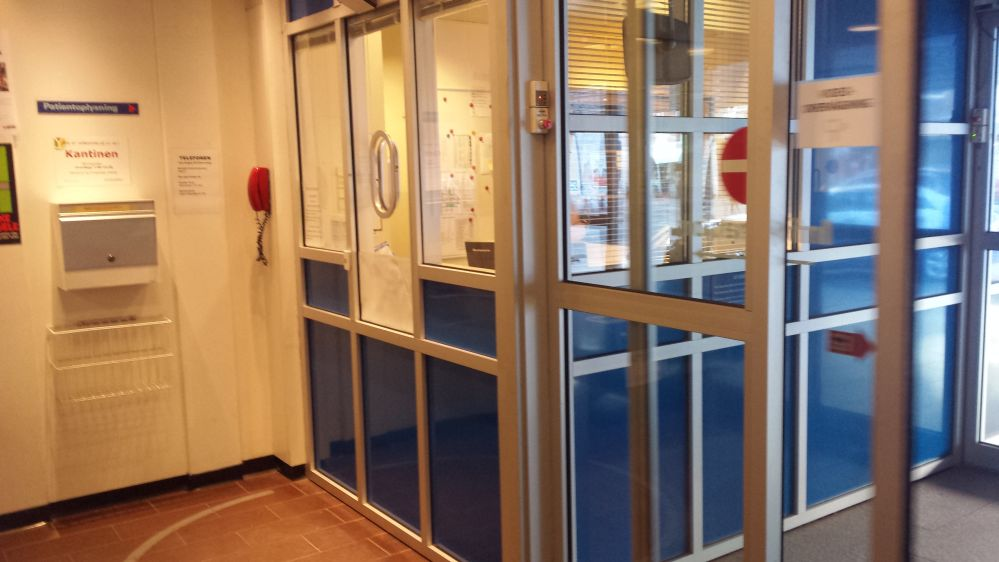
\includegraphics[width=90mm]{reception.jpg}
    \caption{A receptionist booth, seen at Sygehus nord Aalborg}
    \label{fig:rec_booth}
  \end{figure}

\subsubsection{Summary} % (fold)
  We found that in order to have a good navigation platform, the platform needs to be fast to interpret (\cref{sub:sign}), give a fast overview (\cref{sub:map}), be precise (\cref{sub:human}) and easy to understand (\cref{sub:col}). The design of our product has to avoid the weaknesses we have discovered in \cref{sec:anal_nav}. This means that the product must not display irrelevant information (\cref{sub:sign}), must deal with the representation of multiple floors in a non-confusing way (\cref{sub:map}), must deal with positioning without user interaction (\cref{sub:map}), and must be efficient in man hours to maintain (\cref{sub:pho}).

  \chnote{Beginning prerequisites/needs?}

  



%!TEX root = ../../Master.tex
\section{Individual Stakeholders of Indoor Navigation in Hospitals} % (fold)
\label{sec:interusers}

\kanote{mangler der kilder?}

To understand the need for an indoor navigation system, one need to understand the different potential users groups and their needs for an optimized system. The following segment will try to bring forth the different motivations for wanting a more optimised and personalized navigation system.

When it comes to indoor navigation in a hospital, there are two main groups considered individual stakeholders, namely visitors and patients. These groups have different traits, that might be unique for a single group. However the groups we consider, will only account for the traits acquired while navigating, and not the personal traits of the navigator. So before we describe the differences of our two main groups, we must acknowledge that there are personal traits that might be shared across both of the groups.

Humans have natural differences in their ability to navigate. Some individuals can always tell which way is north, some might lose their sense of direction if they spin in place, and many have a hard time telling left from right, without any visual aid.\cite{naturtalenter} There are also certain groups of individual who are more prone to having difficulties navigating, such as the elderly, disabled individual or individual affected by mind altering substances.\cite{MCI} These groups of individual also share a high frequency of visiting hospitals, and so it is increasingly important to address their needs for navigational guidance.\cite{generel}

<<<<<<< 66be35595c5aeaf2550076e2902a01016316d2e8
It is also important to consider the usage of software by the stakeholders. Many elderly are not accustomed with newer technology, and can often be distrustful and easily discouraged when having to interact with information technologies that they have not encountered before.[kilde8] Also when considering software usage, is the need for a reliable rate of information. Studies show, that most users will start to lose their patience after 5 seconds of waiting. [kilde7] These tendencies needs to be adressed, in order to service a greater number of stakeholders.
=======
It is also important to consider the usage of software by the stakeholders. Many elderly are not accustomed with newer technology, and can often be distrustful and easily discouraged when having to interact with information technologies that they have not encountered before.\cite{gamle_teknologi} Also when considering software usage, is the need for a reliable rate of information. Studies show, that most users will start to lose their patience after 5 seconds of waiting. \cite{ventetid} These tendencies needs to be adressed, in order to service a greater number of stakeholders.
>>>>>>> 0369efa8b5a4572d0514a8589da1189021fe59bb

What follows is a closer look at the different needs and traits of the two main groups.

\subsection{Vistors} % (fold)
 \label{par:vistors}
 
An important trait that all types of visitors can share due to the nature of a hospital, is an elevated level of emotional distress. This is often due to the grief or otherwise sadness towards the illness of whom they are visiting. It can also be caused by other things, such as nosocomephobia (fear of hospitals) or claustrophobia (fear of confined spaces, such as elevators) which many individual have a variating degree of.\cite{individforskellige} These traits can all be impairing, if one requires a focused mind when navigating, and it is important to take this into consideration when designing a navigation system. There are two types of visitors that we would like to focus on here, that being those who frequent hospitals and those who do not.

<<<<<<< 66be35595c5aeaf2550076e2902a01016316d2e8
Visitors who do not frequent hospitals, and thus will not have any prior knowledge of the standard infrastructure, will have a hard time navigating the hospital. These visitors will often not be used to navigate any large building, and therefore stationary maps or other guidelines that entails a multitude of actions, which requires memorization, can be hard to adapt to. They will usually prefer asking members of the staff, or using the more simplified yet inefficient forms of navigation, such as counting room numbers or being guided by a friend through a telephone. They will often need confirmation on their current whereabouts and the next course of action.[kilde2 and 5]
=======
Visitors who do not frequent hospitals, and thus will not have any prior knowledge of the standard infrastructure, will have a hard time navigating the hospital. These visitors will often not be used to navigate any large building, and therefore stationary maps or other guidelines that entails a multitude of actions, which requires memorization, can be hard to adapt to. They will usually prefer asking members of the staff, or using the more simplified yet inefficient forms of navigation, such as counting room numbers or being guided by a friend through a telephone. They will often need confirmation on their current whereabouts and the next course of action.\cite{naturtalenter}\cite{individforskellige}
>>>>>>> 0369efa8b5a4572d0514a8589da1189021fe59bb

Visitors who do frequent hospitals, might still share some of the troubles of the non-frequent visitors, but they will however often know, in which quarters the patient they are visiting is situated, and how to get there. But unlike most visitors who do not frequent the hospital, these do not always prepare their visit in full detail, since they might be visiting multiple times a week or even daily. An example of this, could be a parent of a hospitalized child, who decided to drop in during their lunch break. However it just so happened to be, that a part of a doctor's schedule was freed up, and now the child is in another ward, receiving treatment an hour prior to the original schedule. Suddenly, a short visit turns into something much more, because the parent does not necessarily know the details of the rescheduling. Having a loved one confined in a hospital can already be an immense emotional stress factor, but also having to deal with navigating to shifting whereabouts, can easily cause unnecessary agitation.

\subsection{Patients} % (fold)

Patients who either live at the hospital for extended periods or patients who visit the hospital on a weekly or even daily basis, are considered frequent patients. Emergency patients or patients with a non-recurring medical issue, will be considered non-frequent patients. The latter of the two groups, share a significant amount of traits with the normal visitors, but there are some traits that are more common for patients.

A lot of patients are, by the nature of being a patients, not completely well. Many patients will not have their ability to navigate impaired by their medical condition, but for other it can be greatly reduced, sometimes to the point of non-existence. This could include anything from physical injuries such as broken bones or other conditions that confines a patients his beds, or it could be cognitive disabilities either chronic or temporarily medicinally induced. Other disabilities such as visual impairment and dyslexia will often render a visually based guidance system, such as maps, signs and arrows, to be of no virtual help.\cite{visual_impairment}


\subsection{Summary}

These are suboptimal conditions for a facility working with something as important as human lives, and niether medical nor other staff should be required to handle the stress of visitors and paitents, who are having trouble navigating.


% section Interessents - Users (end)

%!TEX root = ../../Master.tex
\section{Organization} % (fold)
\label{sec:organization}

\subsection{Adminitration}

Hospitals have many different kinds of users, in this section the focus is the administrative group; namely the regular staff, the board of directors and The region. All three groups have different traits and impacts on the hospital. \\ The focus in this section is what impact indoor navigation has on the general effectiveness of the hospital and the three groups of administrative staff.\\
Hospitals can involve large and complex buildings \cite{wifi_navigation_ca} and welcomes numerous people every day. Some of those people are patients and others are the loved ones of those patients come to visit, some of whom may be entering for the first time. People who are not used to a hospital can become stressed or confused as they attempt to find an appointment, the cafeteria or the waiting rooms. As a consequence of this they ask the administrative staff for help. \cite{Frivillige_guider}

\textbf{Regular staff}: This group can be split into several subgroups containing for example the receptionist and the administrative assistant. Members of the administrative staff are often the first employees visitors will meet in a hospital, and these employees can be split into two groups in terms of how well they know the building; the new employees and the veteran employees. A new staff member may have a hard time navigating visitors or patients around in a complex facility due to a lack of knowledge of the area, whereas the veteran staff should be more knowledgeable of the facility. Even so it can still be difficult to explain a route through the facility to a visitor. Explaining it is time consuming and it will interrupt what else they might have been working on which in turn may be stressful for the staff \cite{arbejdsmiljo_ca}. If people visiting the hospital are to rely on the staff for navigation it also possesses a bottleneck as each employee can only communicate with one person at a time.

\textbf{Board of Directors and The region}: This group can be split into several subgroups containing for instance, economy and scheduling and quality, normal these groups, don't meed up with the visitors directly, but these groups are Indirectly affected by the visitors and the staff. if staff are on a tight schedule, and they run into an unforeseen workload, then their schedule will slip. this can effect appointments the staff may have. The staff will then have to work overtime, and they will then have to be paid more, effecting the economy in the hospital. A ineffective hospital will cost more money for the region, and the work will / may be of lower quality, this can prevent that the money could be used for something more useful \cite{timer_til_at_hjelpe_rundt}.

In the following we will cover which procedures are needed in order to realize a software solution for our initiating problem (\cref{sub:init}).

In a decision process the following phases will typically happen. \cite{Sjaelland}


\begin{itemize}
  \setlength{\itemsep}{1pt}
  \setlength{\parskip}{0pt}
  \setlength{\parsep}{0pt}
	\item \textbf{Idea and initiative phase} A problem is defined by the citizens, media or political organisation.
	\item \textbf{Preparing phase} The problem will be reviewed according to the health legislation.
	\item \textbf{Decision phase} The problem is presented and a committee is established. This committee will typically work with consultants to specify the requirements of the solution.
	\item \textbf{Implementation phase} The solution will be implemented. 
\end{itemize}

The highest court of the hospital is politically elected bodies: parliament, government and the minister-led ministries and the Regional Council. This was also the Regional Council on 21 September 2010 adopted Region North Jutland budget for 2011 and a budget conciliation, which included a number of structural changes and cost savings for the hospitals in the region \cite{politisk_styret_ca}. Between the decision phase and the implementation phase, the project will be announced as a public supply contract for suppliers to tender. \cite{Union2004}. Suppliers will then submit their solutions. The solution that fits the problem's requirements best, gets the contract. 



In order to create a good navigational system for a hospital, certain factors must be considered. When deciding new features for a hospital, installation \& maintenance costs and compatibility with the existing hardware are big subjects. Therefore this section will describe how the existing infrastructure in hospitals is and how this will affect the navigational system.

\subsection{Wi-Fi} \label{orgwifi}

Most hospitals have good Wi-Fi coverage in the facility. A visit to \enquote{Sygehus Nord} in Aalborg revealed that multiple locations around the hospital had a sufficient amount of Wi-Fi hotspots in range, in order to be used in Location Based Services. See \cref{fig:wifi1,fig:wifi2,fig:wifi3}.

\begin{figure}
\centering
  \begin{minipage}{0.45\textwidth}
    \centering
    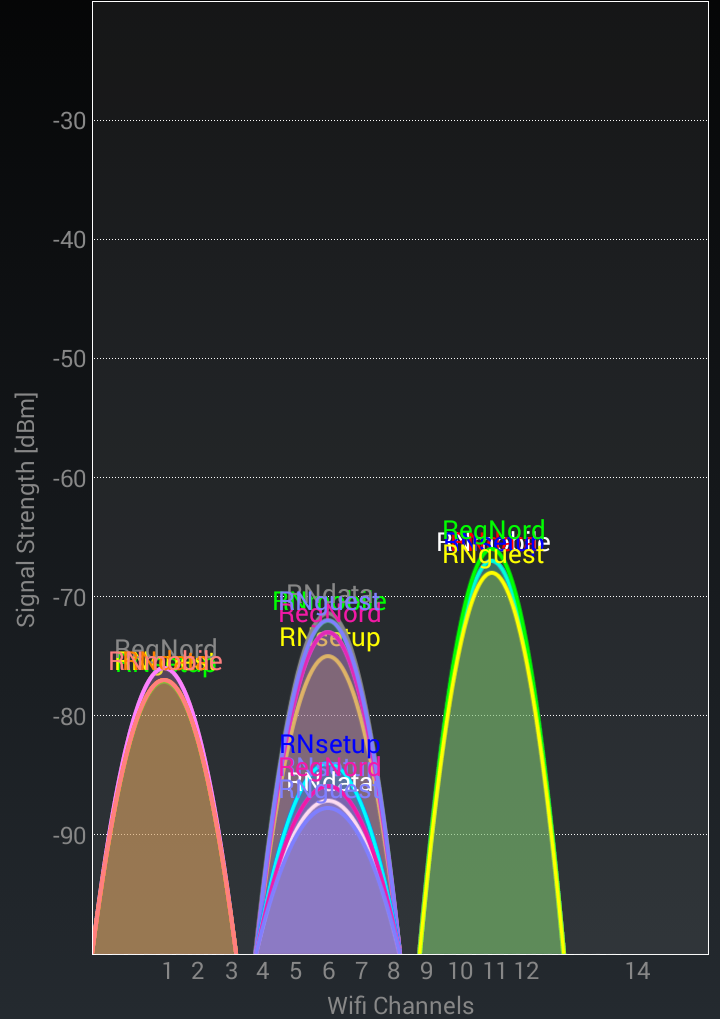
\includegraphics[width=\textwidth]{wifi_sygehus_nord1.png}
    \caption{Graph of signal strength grouped by channels. Location A} \label{fig:wifi1}
  \end{minipage}
  \hfill
  \begin{minipage}{0.45\textwidth}
    \centering
    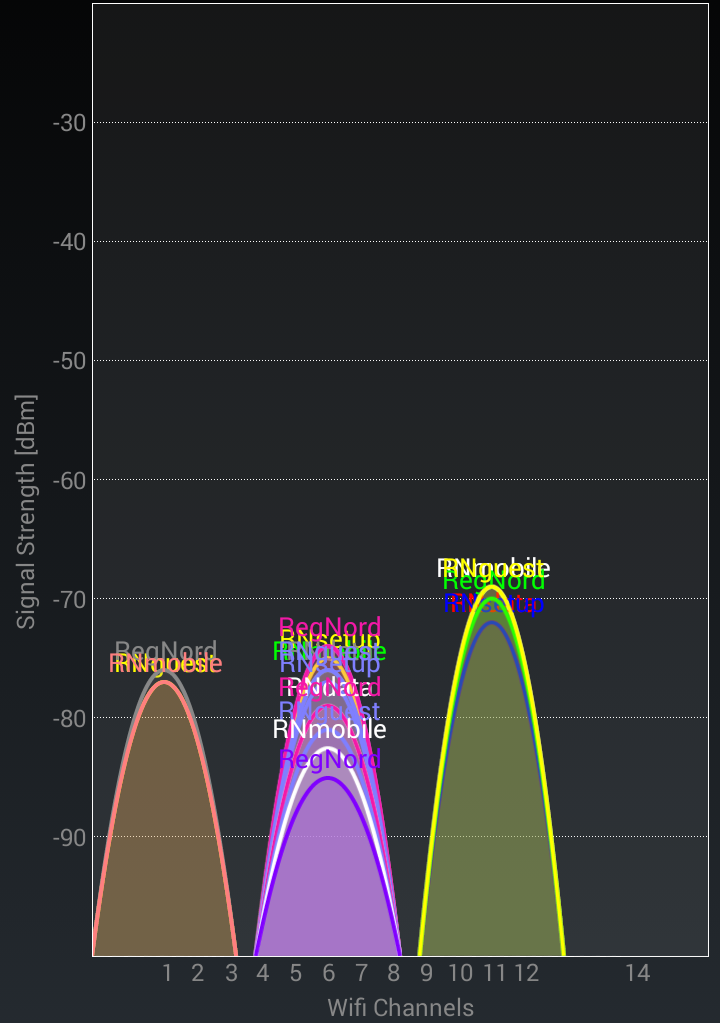
\includegraphics[width=\textwidth]{wifi_sygehus_nord2.png}
    \caption{Graph of signal strength grouped by channels. Location B} \label{fig:wifi2}
  \end{minipage}
    \begin{minipage}{0.45\textwidth}
    \centering
    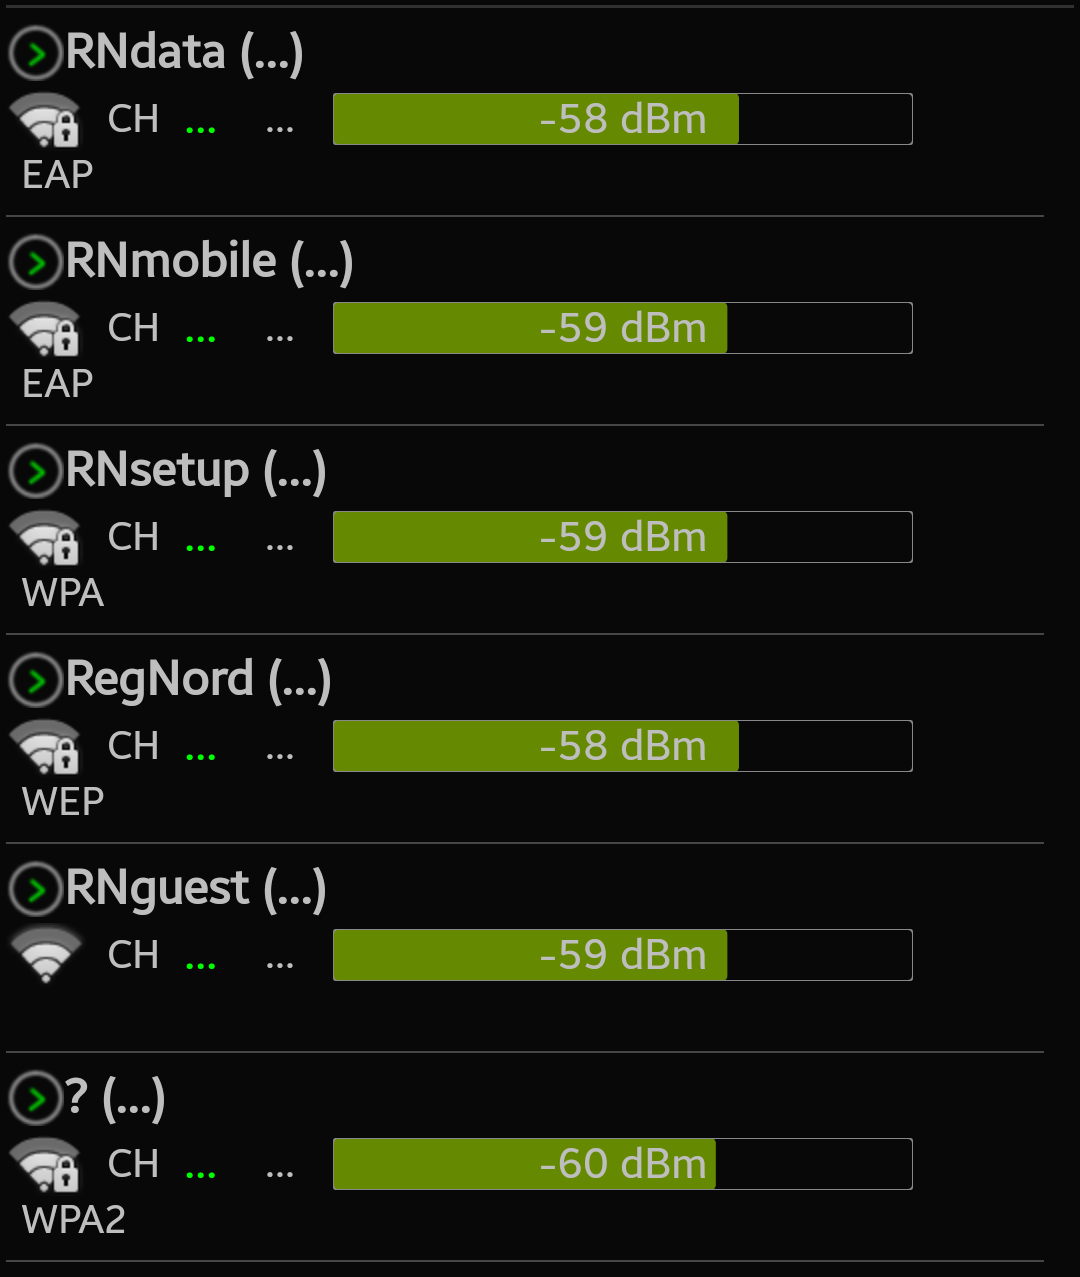
\includegraphics[width=\textwidth]{wifi_sygehus_nord3.png}
    \caption{List of WiFi networks} \label{fig:wifi3}
  \end{minipage}
  \end{figure}


\subsection{Interference with medical device}

Incidents of radio frequency interference between cellular phones, radio broadcasters, WiFi devices and medical devices have been reported. Older models of pacemakers, defibrillators and hearing aid devices were being influenced by near encounter of cellular phones causing undesirable effects like not having control of heartbeat etc. 
The problem was that radio frequency fields were interfering with medical equipment. This has however now been addressed in modern standards, meaning that interference with medical devices does not occur any more. \cite{Man1998,Case}

\subsection{Temporary out-of-order elements}

When mapping a hospital every hall building, stair, elevator etc. has to be considered. Situations may however occur in which some of the mapped elements in fact are temporary out-of-order. This could be an elevator or a hallway being repainted. Updating the navigation system map to include the temporary elements could be a lot of effort. In a situation in which an user of the navigation system is guided through an out-of-order element, the user will most likely find their own way around this obstacle. When this happens, the user is going off-route. The navigation system must support this and act accordingly.

\subsection{Cross-building support}

\canote{de billeder af wifi står da lidt ud af kontest}

Some hospitals will undoubtedly have several building complexes around their cadastral. A good navigational system should work across these platforms providing one, uniform experience. This is both good for the end-user, but as the navigational system can be reused also eases the installation. If support for cross-building complexes has been laid, this could further expand to the navigation system supporting different hospitals independent of each other. The navigation system could then e.g. be installed in all the hospitals in Region Nord, providing an uniform experience for end-users.

\annote{Der mangler et summary til organization}
% section organization (end)

%!TEX root = ../../Master.tex

\section{Technology} \label{tech}

% \kanote{Der efterfølgende stykke har jeg ikke skrevet. Jeg synes godt vi kan beholde meningen, og så bare skrive det om, så vi indlejrer definitionerne, og ikke referer til andre steder? OGSÅ: ideen om at kort beskrive aspekterne af navigation er godt, men skal det stå her?}
% In order to navigate individuals indoor, it is important to always find the most optimal route based on the users prerequisites. This makes wayfinding technologies very important to our project, and we will cover this in \cref{sub:way}. For any wayfinding technique two parameters is required: a start and an end location. The start location can be determined by positioning the individual. This is done using the methods described in \cref{sub:pos}. Positioning have some requirements that the infrastructure has to comply with, we will define those requirements in \cref{sub:infra}.

Before anyone can develop an optimal solution to a problem, it is necessary to understand the technology at one's disposal. But since understanding technology is time consuming, it is important to analyse which to focus on. In the following section, we have selected the technologies that we estimated have the most relevance to our problem, and analysed how they might be used in a possible software solution. It is important to note, that we have only analysed technologies, that support a possible solution to the entirety of our problem, with a few exception. These exceptions have been included because their hold a prominent role in a common optimal solution to a similar problems.

The analysis of the technologies follows a certain simple method. We describe the different existing digital technology, and analyse their relevance to our initiating problem. We then outline the function of a given technology, and determine its relevance by examining why the technology is in use, and specifically which traits makes the technology relevant for our problem. We subsequently describe any undesirable traits which will decrease the usefulness in a possible solution.

\subsection{Method} \label{sub:techmethod}
This method gives a good overview of the usefulness of the given technology, without going into much detail. Details, that are deemed important for understanding a solution or is not otherwise easily obtainable, will be included in a later theoretical chapter.




%Teknologier der kan medtages (HVAD & HVORFOR, IKKE HVORDAN): GPS, RFID, QR-kode, Google Maps, Smartphones, Tablets, PDA, Handheld computing/tracking device, accellerometer, WiFi og andre relevante ting.

%!TEX root = ../../Master.tex
\sinote{Afgræns i afgrænsningen; vi vil kun arbejde med software med øje til handheld devices}

\subsection{Handheld Devices} % (fold)
\label{sub:device}

% subsection subsection_name (end)
 	 
Handheld computing/tracking devices, such as smartphones, tablets and PDAs, are all relatively small and users are able to carry them around. Such devices have a screen, with the exception of some older PDAs, and a Wi-Fi or Bluetooth connection module, that allows them to send and/or receive data. This data can then be projected onto the screen, to inform the user.

%The PDA functions as a personal digital assistant, who will keep track of the user's calender or have a calculator program. Two popular PDA's are the iPod touch and BlackBerrie which are still in use. 
%The Smartphone are much alike the PDA, but have other features such as the ability to receive or make phone calls. Smartphones also a varity of apps that allows 3rd party programs to be installed. Such programs could be digital games or social media programs like Facebook or Twitter. Two popular smartphone series would be the iPhoneor the Samsung galaxy.
%The Tablet is bigger in size compared to the PDA and smartphone, and won't fir in the users pocket. They serve almost the same purpose as the smartphones but have more computing power and memory storage. The tablets are used to satisf the needs that laptop covers that a smartphone will not do competent enough. Such needs could be to surf the world wide net, which many do on their laptop or home PC. This can be done on a smartphone but the screen is often seen as too small. The tablet have a bigger screen and thereofre provides a better experience. Two popular tablet would be the iPad and the Surface. 
Devices like smartphones and tablets are already in use, and they are very popular. This means that for many users, a solution with a downloadable program or application, would be easily adapted. Other navigation programs/applications that they have already used, could have similarities with the solution used in this project, which will ease apdaption even more. These devices are also very portable and can be taken to the hospital without much effort. They can also be used to render a map or otherwise assist the user with navigation, for instance through text, sound or pictures.

For these devices to be used as intended, they requires some prior basic digital knowledge. In order to use the device to navigate trough a given method, the user would have to start the device and navigate to the appropriate application in order to get started. This could potentially hinder some users as this could be confusing to them.

One of the caveats of handheld devices is the limited battery capacity. The battery time of a device depends on many factors including screen-on time, processor usage, radio modems etc. As an example a widely used handheld device has a rated \enquote{internet use} battery time of up to 10 hours. \cite{Apple}

When designing the navigation system the limited battery capacity of these handheld devices must be taken into account.
%The modern devices are also fairly expensive which could make them less attractive to users.

%!TEX root = ../../Master.tex
\subsection{Google Maps}
Google Maps is a web mapping service hosted by Google inc. The application is used by some of Google's other products such as Google Transit\cite{Goo_transist}. 

When a user is using on the Google maps application, all information will be downloaded to their device. Information is downloaded when they search on a location or when they drag the map around\cite{Goo_input}. The satellite images are acquired from other companies like Tele Atlas\cite{Goo_Tele} or Zenrin\cite{Goo_Zenrin} and then overlayed with Ground truth\cite{Goo_GT}.
The map will be shown with a top down view like many other maps and will offer satellite images, road maps or dynamic maps. It is also possible to go into Street View which is another Google tool, from where the viewpoint is from the street level\cite{Goo_street}.

Google maps can be used to plan routes, show earthquakes and even lets you swim with turtles\cite{Goo_Turtle}.

Google maps is relevant for this project as they have made it able to show maps inside buildings, as seen at Aalborg Universitet, Cassiopeia\cite{Goo_Indoor}. This system could be implanted at the hospital so it would show the different floors and have them all mapped. Instead of using a GPS, Google Maps Indoor uses Wi-Fi hotspots and telephone towers to locate their target\cite{Goo_Indoor}.

It is not certain that every complex has enough Wi-Fi hotspots or telephone towers nearby. Therefore this may not be a general solution.

%!TEX root = ../../Master.tex
\subsection{Location Fingerprinting}
In location fingerprinting, there are to main tecniques that have been choosen for this project. It is "QR-code" and "RFID".
Location fingerprinting is method of recognizing devices by giving them a electronic fingerprint, such as a unique id.

\paragraph{QR-code} % (fold)
QR-codes are barcodes that returns data when scanned. The code is represented by black boxes on a white square grid background. All by how the boxes are arranged, the code will represent different data.

In order to read the data, a scanner has to be used. A camera from a smartphone can be used for this purpose, as long there are an app that supports this particular format. Such apps can be found on nearly all smartphones\cite{QR_smart}. The QR-code can be used to lead users to websites, and are used often in different kind of commercial ways\cite{QR_url}.

It is easy to read the QR-code if you already have an app installed on your smartphone. It is also easy to make your own codes as Google have released a free tool to generate them\cite{QR_Google}.It is also rather easy to set up a QR-code system in a effective way\cite{QR_easy}.

The relevance for this project is how it will take little to no time to set up\cite{QR_rel1}, and how some people already knows how use them as they are widely spread\cite{QR_spread}. Even if a code is damaged it will still be usable, all up to 30\% of the code can be missing\cite{QR_dama}. This also means it will be possible to implant images in the code and still have it working\cite{QR_image}.

A reason for not to use the codes could be that some users might exploit the system. If they print their own codes with links to certain websites it could be a very unpleasant experience for the other users\cite{QR_urlbad}. In worst case scenarios they could be used to steal personal information\cite{QR_information}.
In order for the codes to be efficient, they also have to placed at many locations at the hospital. The users should always be able to find them when they want to use them. This could leave to frustration if they seems to be nowhere to find for the user.


\paragraph{RFID}
RFID (Radio Frequency Identification) is a radio technology that makes it possible, just like barcodes, to identify different objects. the main difference between these two technologies is that the barcode is a line of sight technology, and RFID is wireless, as long as it is within visible distance. The readable distance varies depending on the type of RFID tag. The information exchanged can be in many different formats such as text, numbers, audio or video. It depends on the size of the RFID tag built-in memory. 

There are, different RFID tags, as they can be passive, active or battery-assisted. Tags can be read-only "one time read" or read-write "multiply times", have a serial number, or can be plank for the owner to write something on it. To put it into perspective to our project, a read-only tag can be used to find an object such as a printer that does not change its name or property. Read-write tag, can be used to track patients, the information can chance the name and CPR number to match the person who wears it.  


%!TEX root = ../../Master.tex
\subsection{Accelerometer}

The Accelerometer is a transducer that measures acceleration. The acceleration could be static if the device is at hold an only affected by gravity, or dynamic if it moves around\cite{acc_engi}. Accelerometers is used in many different ways and are also used in a lot of different applications, such the PlayStation 3 DualShock 3 remote\cite{acc_ps3} or in a Nokia 5500 sport\cite{acc_nokia}.


The accelerometer is able to detect vibrations, change of altitude or direction\cite{acc_engi}. Some accelerometers works by relying on the piezoelectric effect that delivers electronic output from a variety of crystals inside the device\cite{acc_piezo}. This electronic output can then be read by a computer and used to generate information about the state of the accelerometer.


The accelerometer is among other used because it can reliable be applied in car GPS systems. It uses the technique dead reckoning that estimates ones position based on previously coordinates and current vector movement\cite{acc_dead}. The accelerometer has also proven itself useful in some science aspects, such as earthquake investigations or monitoring active volcanoes\cite{acc_vulkan}. 


The accelerometer is relevant for this project, as it can be used to position the users if it is incorporated in a device that is going to be carried along side the current user. In this way it could be used to see if the user is following the generated path or if he/she have moved outside of it. The accelerometers that could be used for this project could be the LIS302DL as it is rather cheap and compact\cite{acc_price,acc_lis302dl}. This accelerometer have already been incorporated in the original iPhone\cite{acc_iPhone}.


A downside with the accelerometer is that it can not stand on its own. The accelerometer is unable to position itself and will therefore need to work alongside another system, such as a GPS or wifi and etcetera. 

\subsubsection{Wi-Fi} \label{wifitech}
Wi-Fi is a technology that uses radio waves to transfer data between electronic devices. Computers and handheld devices make use of Wi-Fi, together with many other electronic devices \cite{wifi_devices}.

Wi-Fi can be used in location fingerprinting using triangulation. This works because every Wi-Fi hotspot has an unique id and a known location. An estimated position of a Wi-Fi receiver can be calculated based on the signal strength to every Wi-Fi hotspot. It is then possible to calculate a position  \cite{Liu2007}.

Wi-Fi can connect to the internet via a wireless access point such as a router. Wi-Fi allows places that normally would not have internet connection, like sheds or gardens, to connect. This is possible as the router or wireless access point will allow the device to get a connection.

This is widely used as they serve as an convenient way of getting internet access. They are fairly easy to set up and used widely in the private homes and also used at a greater scale such as an airport \cite{wifi_works}. It is an convenient way of getting internet access as the user is in no need of getting a cable that physically have to be connected to a router.

It is relevant for this project as there have been invested in installing Wi-Fi hotspots at the Danish hospitals \cite{wifi_hospi}. This means it would be possible to set up a service that will connect trough these hotspots.

A problem with Wi-Fi is how, as by Danish law, the hospital will have to log data from the users who connect to it \cite{wifi_log}. In order to only log the users who are using the Wi-Fi, a password would be optimal as it will prevent people bypassing the complex from automatically connecting. The range is also a limitation as typical routers will support a range of 46 meters indoor \cite{wifi_range}. Walls will reduce the strength of the signal, which means some areas of the complex might no have a good enough connection \cite{wifi_wall}. Handheld devices consumes more power when Wi-Fi is active, and quickly drains the battery as data is send and received \cite{wifi_batt}. The amount of power used is reduces as the device goes into a low power mode, which is activated once it has no more data to send. It goes into hight power mode when it is sending/receiving data and stays there for the duration of which it is sending/receiving the data.


%!TEX root = ../../Master.tex

\subsection{GPS}

Global Positioning System, GPS is a satellite-based positioning system. Satellites emits a signal, a time-stamp and current position. A GPS receiver measures the distance from itself to any satellite, by the time it took to receive the signal at the speed of light. When the positions and distances of multiple of satellites is known, its possible determine the GPS receivers position by trilateration \cite{Dempster2013}. It is possible to use GPS all over the world as long as there a clear line of sight to the satellites. Due to the signals not being able to pass through walls and roofs, means that it is suitable for indoor use \cite{GPS_about}.

 
%%!TEX root = ../../Master.tex


\subsection{Positioning}\label{sub:pos}

  Triangulation is a method used for estimating the position of an object. The method uses the properties of triangles. Triangulation has two derivatives: literation and angulation.

 \subsubsection{Lateration}

  Lateration is commonly used technique for positioning.  Lateration uses the distance between known locations and and the point to be determined, to estimate the location.\cite{tri_lateration}  There are two types of lateration two dimensional and three dimensional. The two dimensional are use in robots that navigates in only one plane, like robot vacuum cleaners. 
  lateration in three dimensions are used in GPS positioning, and other practical applications for positioning.

  \subsubsection{Angulation}

  Angulation uses the technique called Angle of Arrival (AOA), which can compute the location of a source. The parameters needed are as minimum two relative angles between a remote point and the source, and the distance between the remote points. The source is at the location where the lines formed by the angle direction lines intercept. 

  In 2D, as few as two remote points are needed, given the source is not directly in between the remote points. However to improve accuracy and remove ambiguity  another remote point is needed. In 3D, as few as three remote points are needed. However as with 2D, another remote point improves accuracy and removes ambiguity. \cite{Liu2007, Sun2009, Boontrai2009}


  \subsubsection{Location Fingerprinting}


  Location fingerprinting is another techinque used for positioning. It refers to the algorithms that first collect characteristics (fingerprints) of a scene and then matches these a priori characteristics with the characteristics of the location the source is in, to determine the source' location.

  There are two stages for location fingerprinting. The offline state where a site survey is performed in the environment. The characteristics of known locations are stored in databases. In the online state, these a priori characteristics are used to match the location of the source.

  The main challenge of location fingerprinting is the possibility of variating signal strengths corrupting characteristics data.

  \subsubsection{Summary}


  All of the above described technologies need remote points to find a position. As described in \cref{sub:infra}, many hospitals have WiFi hotspots located around the hospital. These WiFi hotspots can be used as the remote points, given that the coverage of the network is good.
